%! Author = kubec
%! Date = 06.03.2024

% Preamble
\documentclass[11pt]{article}

% Packages
\usepackage{amsmath}
\usepackage{mathtools}
\usepackage{ragged2e}
\usepackage [utf8]{inputenc}
\usepackage{blindtext}
\usepackage{wrapfig}
\usepackage{xcolor}
\usepackage {polski}
\usepackage{multicol}
\usepackage[a4paper, total={5.7in, 8in}]{geometry}
\usepackage{graphicx}
\usepackage{amstex}
\usepackage{csvsimple}
\usepackage{changepage}
\usepackage{enumitem}
\usepackage[english]{babel}
\usepackage{biblatex}
\usepackage{caption}

\addbibresource{bibliografia.bib}


% Document
\begin{document}
%    Tytuł
    \begin{flushright}
        \large{
            Igor Czerwiec - 277680\\
            Filip Kubecki - 272655
        }\\
    \end{flushright}
    \begin{center}
        \large{Fizyka 3.1}\\
        \vspace{2mm}
        \LARGE{\textbf{Wyznaczanie gęstości ciał stałych}}\\
        \vspace{3mm}
        \huge{Nr ćwiczenia: 100a}\\
        \vspace{1cm}
    \end{center}
    \begin{flushright}
        \large{
            Data wykonania ćwiczenia: 07.03.2024r\\
            Data oddania sprawozdania: 13.03.2024r
        }\\
    \end{flushright}
    \vspace{1cm}
%    Część główna
    \section{Wstęp}
    \par{
        Celem zadania jest wyznacznie gęstości dwóch elementów poprzez pomiar ich wymiarów fizycznych, obliczenie objętości i zmierzeniu ich mas.
        Ćwiczenie ma za zadanie zapoznać eksperymentatorów z metodologią przeprowadzania pomiarów wielkości fizycznych oraz analizy niepewności.
    }
    \vspace{3mm}
    \par{\noindent \textbf{Wykorzystane przyrządy pomiarowe:}}
    \begin{itemize}[topsep=0pt]
        \itemsep0em
        \item Suwmiarka (błąd pomiarowy 0.05 [mm])
        \item Mikrometr (błąd pomiarowy 0.01 [mm])
        \item Waga (błąd pomiarowy 0.01 [g])
        \item Cylinder miarowy (błąd pomiarowy 1 [ml])
    \end{itemize}
    \vspace{3mm}
    \par{\noindent \textbf{Przebieg doświadczenia:}}
    \par{\noindent
    Za pomocą suwmiarki oraz mikrometru zmierzono kolejne wymiary elementów (tulei oraz wałka).
    Pozwoliło to na wyznaczenie ich objętości przy użyciu poniższych wzorów:
    }
    \begin{gather*}
        V = \pi L(R^2 -r^2)\\
        V =  \sum_{n=1}^{5}(l_n\pi {r_{n}}^2)-l_x\pi {r_{x}}^2
    \end{gather*}
    {
        \footnotesize
        \begin{itemize}
            \setlength\itemsep{0.1em}
            \item[] $V$ - objętość elementu,
            \item[] $L/l_n/l_x$ - kolejne pomiary długości,
            \item[] $R/r/r_n/r_x$ - kolejne pomiary promienia,
        \end{itemize}
    }
    \par{\noindent
        Następnie został wykonany pomiar masy za pomocą wagi laboratoryjnej. 
        Na podstawie uzyskanych danych można wyznaczyć gęstość elementów za pomocą wzoru:
    }
    \begin{gather*}
        \rho=\frac{m}{V}
    \end{gather*}
    {
        \footnotesize
        \begin{itemize}
            \setlength\itemsep{0.1em}
            \item[] $\rho$ - gęstość elementu,
            \item[] $m$ - masa elementu,
            \item[] $V$ - objętość elementu,
        \end{itemize}
    }
    \begin{figure}
        \centerline{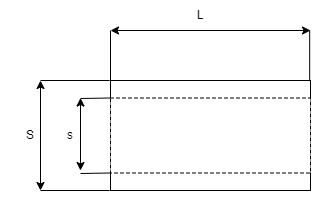
\includegraphics[scale=.6]{tuleja.drawio.png}}
        \caption*{Wymiary tulei}
    \end{figure}
    \begin{figure}
        \centerline{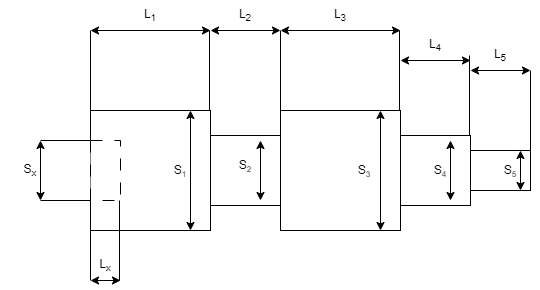
\includegraphics[scale=.6]{walek.png}}
        \caption*{Wymiary wałka}
    \end{figure}

    \newpage
    \section{Dane}

%    \csvautotabular{Dane100aCylinder.csv}
    \subsection{Pomiary tulei}
    \begin{center}
        \csvreader[tabular = |c|c|c|c|c|,
            table head = \hline \textbf{Masa[g]} & \textbf{L[mm]} & \textbf{S[mm]} & \textbf{s[mm]} & \textbf{V[ml]}\\\hline,
%            table foot = \hline,
            late after line = \\\hline
        ]{Dane100aCylinder.csv}{}{
            \csvcoli & \csvcolii & \csvcoliii & \csvcoliv & \csvcolv
        }
    \end{center}

    \subsection{Pomiary wałka}
    \begin{center}
%        \csvautotabular{Dane100aWalek.csv}
        \csvreader[
            tabular = |c|c|c|c|c|c|c|,
            table head =  \hline \textbf{Masa[g]} & \textbf{L1[mm]} & \textbf{L2[mm]} & \textbf{L3[mm]} & \textbf{L4[mm]} & \textbf{L5[mm]}& \textbf{Lx[mm]}\\\hline,
%            table foot = \hline,
            late after line = \\\hline
%    late after line = \\\hline
        ]{Dane100aWalek.csv}{}{
            \csvcoli & \csvcolii & \csvcoliii & \csvcoliv & \csvcolv & \csvcolvi & \csvcolvii
%
        }
    \end{center}
    \begin{center}
%        \csvautotabular{Dane100aWalek.csv}
        \csvreader[
            tabular = |c|c|c|c|c|c|c|,
            table head = \hline \textbf{S1[mm]} & \textbf{S2[mm]} & \textbf{S3[mm]} & \textbf{S4[mm]} & \textbf{S5[mm]} & \textbf{Sx[mm]} & \textbf{V[ml]}\\\hline,
%            table foot = \hline,
            late after line = \\\hline
        ]{Dane100aWalek.csv}{}{
            \csvcolviii & \csvcolix & \csvcolx & \csvcolxi & \csvcolxii & \csvcolxiii & \csvcolxiv
        }
    \end{center}

    \section{Obliczenia}
    \subsection{Tuleja}
    \noindent Niepewność pomiarową przyrządów pomiarowych (niepewność standardowa typu B) obliczamy ze wzoru:
    \begin{gather*}
        u_b(\Delta)=\sqrt{\sum_{i=1}^{n}\frac{(\Delta_i)^2}{3}}
    \end{gather*}
    {\footnotesize
        \begin{itemize}
            \item[] $\Delta_i$ - kolejne błędy pomiarowe np: przyrządu, obserwatora,odczytu wartości tablicowych itd,
        \end{itemize}}
    \noindent Przykładowo dla niepewności pomiarowej mikrometra:
    \begin{gather*}
        u_b(\Delta_m)=\sqrt{\frac{(0.01[mm])^2}{3}}=0.00577350\dots[mm]\approx 0.0058[mm]
    \end{gather*}
    {\footnotesize
        \begin{itemize}
            \item[] $\Delta_m$ - bład pomiarowy mikrometra,
        \end{itemize}}

    \noindent Niepewność statystyczna (niepewność standardowa typu A) wielu pomiarów wyliczamy ze wzoru:
    \begin{gather*}
        u_a(x)=\sqrt{\frac{\sum_{i=1}^n (x_i-\hat{x})^2}{n(n-1)}}
    \end{gather*}
    {\footnotesize
        \begin{itemize}
            \item[] $x_i$ - kolejne pomiary danej wielkości,
            \item[] $\hat{x}$ - średnia z wszystkich pomiarów,
            \item[] $n$ - liczba pomiarów,
        \end{itemize}}
    \noindent Przykładowo dla niepewności pomiaru długości L tulei:
    \begin{gather*}
        u_a(L)=\sqrt{\frac{ (36-36.6)^2+(36-36.6)^2+(36.1-36.6)^2+(36.1-36.6)^2+(36.1-36.6)^2}{20}}=\\
        =0.024494897\dots[mm] \approx 0.025 [mm]
    \end{gather*}

    \noindent Niepewność całkowita wyraża się wzorem:
    \begin{gather*}
        u_c(x)=\sqrt{u_a^2(x)+u_b^2(x)}
    \end{gather*}

    \noindent Na przykładzie niepewności całkowitej długości L:
    \begin{gather*}
        u_c(L)=\sqrt{0.025^2+0.029^2}\approx 0.038 [mm]
    \end{gather*}

    \noindent Objętość tulei wyraża się wzorem:
    \begin{gather*}
        V = \pi L(R^2 -r^2)
    \end{gather*}
    {\footnotesize
        \begin{itemize}
            \setlength\itemsep{0.1em}
            \item[] $V$ - objętość wałka,
            \item[] $L$ - Średni pomiar długości,
            \item[] $R$ - Średni pomiar promienia zewnętrznego,
            \item[] $r$ - Średni pomiar promienia wewnętrznego,
        \end{itemize}
    }
    \noindent Podstawiając dane:
    \begin{gather*}
        V =  36.06\pi(8.014^2 - 5.79^2)=3476.12275[mm^3]\approx 3.48 [ml]
    \end{gather*}
    \noindent Niepewność pomiarowa objętości tulei wyraża się wzorem:
    \begin{gather*}
        u(V) = \sqrt{\biggl(\frac{\partial V}{\partial L}\biggr)^2 u_c^2(L)+
                {\biggl(\frac{\partial V}{\partial r}\biggr)^2 u_c^2(r)}+
                { \biggl(\frac{\partial V}{\partial R}\biggr)^2 u_c^2(R)}}=\\
        =\sqrt{{ \biggl( \pi(R^2 - r^2) \biggr)^2 u_c^2(L)}+
                {\biggl(-2Lr\pi \biggr)^2 u_c^2(r)}+
                {\biggl(2LR\pi \biggr)^2 u_c^2(R)}}
    \end{gather*}
    \noindent Po podstawieniu danych otrzymujemy wynik:
    \begin{gather*}
        u(V)=82.06148[mm^3]\approx 0.082[ml]
    \end{gather*}
    \noindent Gęstość tulei wyraża się wzorem:
    \begin{gather*}
        \rho=\frac{m}{V}
    \end{gather*}
    \noindent Po podstawieniu danych otrzymujemy wynik:
    \begin{gather*}
        \rho=0.0025056\dots[\frac{g}{mm^3}]\approx 0.0025 [\frac{g}{mm^3}] = 2500 [\frac{kg}{m^3}]
    \end{gather*}

    \noindent Niepewność pomiarowa gęstości tulei:
    \begin{gather*}
        u(\rho)=\sqrt{\biggl(\frac{\partial \rho}{\partial m}\biggr)^2u_b^2(m)+
        \biggl(\frac{\partial \rho}{\partial V}\biggr)^2u^2(V)}
        =\sqrt{\biggl(\frac{1}{V} \biggr)^2u_b^2(m)+
        \biggl(\frac{m}{V^2}\biggr)^2u^2(V)}=\\
        =\sqrt{\biggl(\frac{1}{3476} \biggr)^2 0.0058^2+
        \biggl(\frac{8.71}{3476^2}\biggr)^2 124^2}=0.00146552[\frac{g}{mm^3}]=\\
        =0,0000894038[\frac{g}{mm^3}]\approx 0.000089[\frac{g}{mm^3}]= 89 [\frac{kg}{m^3}]
    \end{gather*}

    \subsection{Wałek}
    \noindent Objętość wałka dana jest wzorem:
    \begin{gather*}
        V =  \sum_{n=1}^{5}(l_n\pi {r_{n}}^2)-l_x\pi {r_{x}}^2
    \end{gather*}
    {
        \footnotesize
        \begin{itemize}
         \setlength\itemsep{0.1em}
         \item[] $V$ - objętość wałka,
         \item[] $l_n/l_x$ - kolejne pomiary długości,
         \item[] $r_n/r_x$ - kolejne pomiary promienia,
    \end{itemize}
    }
    \noindent Podstawiając dane otrzymujemy:
    \begin{gather*}
        V = 23\ 228.28[mm^3]\approx 23.23 [ml]
    \end{gather*}
    \noindent Niepewność pomiarowa objętości wałka wyraża się wzorem:
    \begin{gather*}
        u(V) = \sqrt{\sum_{n=1}^{5} \biggl(\frac{\partial V}{\partial l_n}\biggr)^2 u_c^2(l_n)+
        {\sum_{n=1}^{5} \biggl(\frac{\partial V}{\partial r_n}\biggr)^2 u_c^2(r_n)}+
        { \biggl(\frac{\partial V}{\partial l_x}\biggr)^2 u_c^2(l_x)}+
        { \biggl(\frac{\partial V}{\partial r_x}\biggr)^2 u_c^2(r_x)}}=\\
        =\sqrt{ \sum_{n=1}^{5} { \biggl( \pi {r_n}^2 \biggr)^2 u_c^2(r_n)}+
        { \sum_{n=1}^{5} { \biggl( l_n \pi \biggr)^2 u__c^2(l_n)}}+
        { \biggl(  \pi {r_x}^2 \biggr)^2 u_c^2(r_x)}+
        { \biggl( l_x \pi  \biggr)^2 u_c^2(l_x)}}
    \end{gather*}
    \noindent Podstawiając dane otrzymujemy:
    \begin{gather*}
        u(V)=34.25533[mm^3]\approx 0.034 [ml]
    \end{gather*}
    \noindent Pozostałe obliczenia analogicznie do obliczeń tulei.

%    Obliczamy gęstośc ze
%    \begin{gather*}
%        \rho=\frac{m}{V}=\frac{64.85[g]}{23200[mm^3]}=0.002795[\frac{g}{mm^3}]=2795[\frac{kg}{m^3}]
%    \end{gather*}
%    Niepewność pomiarowa gęstości:
%    \begin{gather*}
%        u(\rho)=\sqrt{\biggl(\frac{\partial \rho}{\partial m}\biggr)^2u_b^2(m)+
%        \biggl(\frac{\partial \rho}{\partial V}\biggr)^2u^2(V)}
%        =\sqrt{\biggl(\frac{1}{V} \biggr)^2u_b^2(m)+
%        \biggl(\frac{m}{V^2}\biggr)^2u^2(V)}=\\
%        =\sqrt{\biggl(\frac{1}{23200} \biggr)^2 0.0058^2+
%        \biggl(\frac{64.85}{23200^2}\biggr)^2 34^2}=0.00146552[\frac{g}{mm^3}]=\\
%        =0.00000410412[\frac{g}{mm^3}]\approx 0.0000041[\frac{g}{mm^3}]= 4.1[\frac{kg}{m^3}]
%    \end{gather*}
    \section{Wyniki}
    \subsection{Tuleja}
    \begin{center}
        \csvreader[tabular = |c|c|c|c|c|c|,
            table head = \hline & \textbf{M[$g$]} & \textbf{L[$mm$]} & \textbf{R[$mm$]} & \textbf{r[$mm$]} & \textbf{V[$ml$]}\\\hline,
%            table foot = \hline,
            late after line = \\\hline
        ]{WynikiTuleja1.csv}{}{
            \csvcoli & \csvcolii & \csvcoliii & \csvcoliv & \csvcolv & \csvcolvi
        }
    \end{center}
    \begin{center}
        \csvreader[tabular = |c|c|c|c|,
            table head = \hline \textbf{V[$mm^3$]} & \textbf{u(V)[$mm^3$]} & \textbf{$\pmb\rho$[$\frac{kg}{m^3}$]} & \textbf{u($\pmb\rho$)[$\frac{kg}{m^3}$]} \\\hline,
%            table foot = \hline,
            late after line = \\\hline
        ]{WynikiTuleja2.csv}{}{
            \csvcoli & \csvcolii & \csvcoliii & \csvcoliv
        }
    \end{center}
    \subsection{Wałek}
    \begin{center}
        \csvreader[tabular = |c|c|c|c|c|c|c|,
            table head = \hline & \textbf{M[$g$]} & \textbf{L1[$mm$]} & \textbf{L2[$mm$]}& \textbf{L3[$mm$]}& \textbf{L4[$mm$]}& \textbf{L5[$mm$]}\\\hline,
%            table foot = \hline,
            late after line = \\\hline
        ]{WynikiWalek1.csv}{}{
            \csvcoli & \csvcolii & \csvcoliii & \csvcoliv & \csvcolv & \csvcolvi & \csvcolvii
        }
    \end{center}
    \begin{center}
        \csvreader[tabular = |c|c|c|c|c|c|c|c|,
            table head = \hline \textbf{Lx[$mm$]}& \textbf{R1[$mm$]} & \textbf{R2[$mm$]} &\textbf{R3[$mm$]} &\textbf{R4[$mm$]} &\textbf{R5[$mm$]} &\textbf{Rx[$mm$]} &\textbf{V[$ml$]} \\\hline,
%            table foot = \hline,
            late after line = \\\hline
        ]{WynikiWalek1.csv}{}{
            \csvcolviii &\csvcolix & \csvcolx & \csvcolxi & \csvcolxii & \csvcolxiii & \csvcolxiv & \csvcolxv
        }
    \end{center}
    \begin{center}
        \csvreader[tabular = |c|c|c|c|,
            table head = \hline \textbf{V[$mm^3$]} & \textbf{u(V)[$mm^3$]} & \textbf{$\pmb\rho$[$\frac{kg}{m^3}$]} & \textbf{u($\pmb\rho$)[$\frac{kg}{m^3}$]} \\\hline,
%            table foot = \hline,
            late after line = \\\hline
        ]{WynikiWalek2.csv}{}{
            \csvcoli & \csvcolii & \csvcoliii & \csvcoliv
        }
    \end{center}
    \newpage
    \section{Wnioski}
    Z zmierzonych wartości udało się otrzymać następujące gęstości:
    \begin{itemize}
        \item Tuleja - $2506\pm 89[\frac{kg}{m^3}]$
        \item Wałek - $2795.3\pm 4.1 [\frac{kg}{m^3}]$
    \end{itemize}
    \par{\noindent Porównując do wartości tablicowych gęstośc tuleji jest bliska gęstości aluminium podawanej na $2600[\frac{kg}{m^3}]$ gdy uwzględnimy niepewnosć obliczania gęstości.
    Jednak po analizie danych wejściowych regułą trzech sigm można zauważyć że jedna z wartości parametru $s$ nie mieści się w kryterium jest to wiec bład gruby.
    Po usunięciu jej otrzymujemy wartość $2564\pm 89[\frac{kg}{m^3}]$ co wpisuje się w zakres gęstości aluminium z większą dokładnością.}
    \vspace{1mm}
    \par{\noindent Gęstość wałka jest bardzo zbliżona do gęstości duraluminium którego gęstość wynosi $2800[\frac{kg}{m^3}]$ co oznacza że pomiar został przeprowadzony bez większych błedów.}
\end{document}